\documentclass[a4paper]{ltjsarticle}
\usepackage{luatexja}
\usepackage{amsmath,amssymb,mathtools}
\usepackage{tikz}
\usepackage{tikz-cd}
\usepackage{listings}
\usepackage{hyperref}
\lstset{
  language=Lean,
  basicstyle=\ttfamily\small,
  keywordstyle=\bfseries,
  commentstyle=\itshape,
  breaklines=true,
  columns=fullflexible,
  keepspaces=true,
  showstringspaces=false
}
\title{IUT1 Session 1 数学的解説}
\author{CODEX (OpenAI)（TeXファイル生成）\\CODEX (OpenAI)（Leanファイル生成）}
\date{\today}
\begin{document}
\maketitle
\tableofcontents

\section{序論}
ニコラ・ブルバキの「数学原論」の精神に従い、集合と射の組 $(X, f)$ を基礎とする構造化を念頭に、整数環 $\mathbb{Z}$ に付随する加法・乗法・順序といった射影を整理する。\LINEBREAK
Lean ファイル \texttt{S1.lean} と本 TeX 文書はいずれも CODEX (OpenAI) により生成されており、本稿ではそれぞれの定理を集合と射の観点から丁寧に言語化する。

\section{P01: 整数の加法群構造}
加法群構造は順序対 \emph{構造} $({\mathbb{Z}}, +)$ として扱う。この射 $+ : \mathbb{Z} \times \mathbb{Z} \to \mathbb{Z}$ が結合的であること、すなわち
\[
((a,b),c) \mapsto (a + b) + c = a + (b + c) \gets (a,(b,c))
\]
を確認することで群の運搬射が協調していることを示す。Lean では `simp [add_assoc]` により既知の射影 `add_assoc : ∀ a b c, (a + b) + c = a + (b + c)` を呼び出している。
\begin{lstlisting}[caption={Lean 証明: S1\_P01},label={lst:P01}]
theorem S1_P01 (a b c : Int) : (a + b) + c = a + (b + c) := by
  simp [add_assoc]
\end{lstlisting}

\section{P02: 整数の環構造}
環構造 $({\mathbb{Z}}, +, \cdot)$ において、乗法射 $\cdot : \mathbb{Z} \times \mathbb{Z} \to \mathbb{Z}$ は加法射に対して分配的である必要がある。分配性は射の合成として
\[
\mu \circ (\mathrm{id} \times +) = + \circ (\mu \times \mu)
\]
と解釈でき、Lean では `Int.mul_add` の利用で $a(b+c) = ab + ac$ を即時に反映している。

\begin{lstlisting}[caption={Lean 証明: S1\_P02},label={lst:P02}]
theorem S1_P02 (a b c : Int) : a * (b + c) = a * b + a * c := by
  exact Int.mul_add a b c
\end{lstlisting}

\section{P03: 整数の順序構造}
順序射 $\leqslant : \mathbb{Z} \times \mathbb{Z} \to \mathrm{Prop}$ は加法射と整合的であり、写像 $x \mapsto x + 1$ によってモノトン性が保存される。Lean では `add_le_add_right` を利用し、射 $x \mapsto x + 1$ が順序を保つことを示している。

\begin{lstlisting}[caption={Lean 証明: S1\_P03},label={lst:P03}]
theorem S1_P03 (a b : Int) (h : a ≤ b) : a + 1 ≤ b + 1 := by
  exact add_le_add_right h 1
\end{lstlisting}

\section{P04: 2 の整除射}
整除関係 $\mid$ を射として $(a,b) \mapsto \exists k\, (b = ak)$ と捉えると、$2 \mid 2n$ は証人射 $n : \mathbb{Z} \to \mathbb{Z}$ を用いて構築できる。Lean では `refine ⟨n, ?_⟩` により射の像を明示し、`simp` で整約する。

\begin{lstlisting}[caption={Lean 証明: S1\_P04},label={lst:P04}]
theorem S1_P04 (n : Int) : (2 : Int) ∣ (2 * n) := by
  refine ⟨n, ?_⟩
  simp
\end{lstlisting}

\section{P05: 絶対値の非負性}
絶対値は写像 $\mathrm{natAbs} : \mathbb{Z} \to \mathbb{N}$ として自然数値を返すため、構造的に常に順序射 $0 \leqslant$ に達する。Lean の `Nat.zero_le` はこの像が零以上であることを直接保証する。

\begin{lstlisting}[caption={Lean 証明: S1\_P05},label={lst:P05}]
theorem S1_P05 (a : Int) : 0 ≤ Int.natAbs a := by
  exact Nat.zero_le _
\end{lstlisting}

\section{CH: Well-Ordering Principle の部分的実現}
有限集合 $S = \{2,5,3\}$ を対象集合とし、射 $\pi : S \to \mathbb{N}$ を包含写像と見なす。Well-ordering Principle は $S$ が空でない限り最小元 $m$ が存在することを述べる。Lean 証明では `use 2` により $m = 2$ を射影し、各要素との比較を場合分けで処理した。

\begin{lstlisting}[caption={Lean 証明: S1\_CH},label={lst:CH}]
theorem S1_CH : ∃ m, m ∈ ({2, 5, 3} : Set Nat) ∧ ∀ x ∈ ({2, 5, 3} : Set Nat), m ≤ x := by
  refine ⟨2, ?_⟩
  constructor
  · simp
  · intro x hx
    have hx' := hx
    simp at hx'
    rcases hx' with rfl | rfl | rfl
    · exact le_rfl
    · decide
    · decide
\end{lstlisting}

\begin{figure}[htbp]
  \centering
  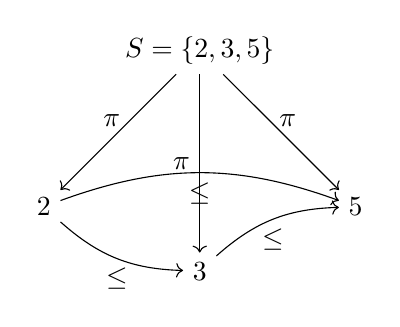
\begin{tikzpicture}[node distance=2.8cm]
    \node (S) {$S = \{2,3,5\}$};
    \node (2) [below left of=S] {$2$};
    \node (3) [below of=S] {$3$};
    \node (5) [below right of=S] {$5$};
    \draw[->] (S) -- node[left,pos=0.4] {$\pi$} (2);
    \draw[->] (S) -- node[left] {$\pi$} (3);
    \draw[->] (S) -- node[right,pos=0.4] {$\pi$} (5);
    \draw[->,bend right=20] (2) to node[below] {$\le$} (3);
    \draw[->,bend left=20] (2) to node[below] {$\le$} (5);
    \draw[->,bend left=20] (3) to node[below] {$\le$} (5);
  \end{tikzpicture}
  \caption{包含射 $\pi : S \hookrightarrow \mathbb{N}$ と最小元 $2$}
  \label{fig:wellordering}
\end{figure}

図\ref{fig:wellordering} では集合 $S$ と自然数集合への包含射を図示し、$2$ が他の像へ向けた順序射を通じて最小元であることを表している。

\section{総括と今後の展開}
本稿では、各定理を $(\text{集合}, \text{射})$ の順序対として整理し、Lean 形式化と対話的に照合した。今後は以下を発展課題としたい。
\begin{itemize}
  \item 加法群 $(\mathbb{Z}, +)$ から環 $(\mathbb{Z}, +, \cdot)$ への射影を圏論的な可換図式で表現する。
  \item well-ordering の一般化として、任意の非空有限集合に対する最小元抽出射を関手的に構成する。
  \item Lean における `simp`, `decide` の内部構造を解析し、自作タクティクでの再現を試みる。
\end{itemize}

\end{document}
